\documentclass[tikz]{standalone}
\usepackage{pgfplots}
\pgfplotsset{compat=1.15}
\usepackage{mathrsfs}
\usetikzlibrary{arrows,calc}
\usepackage{tkz-euclide}
\pagestyle{empty}

\definecolor{AngleClr}{rgb}{0,0.39215686274509803,0}
\definecolor{ShapeClr}{rgb}{0.6,0.2,0}
\definecolor{BlueClr}{RGB}{13,93,184}

\begin{document}

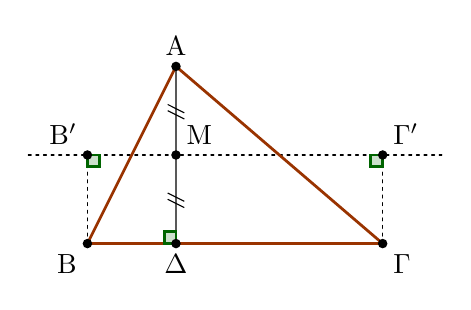
\begin{tikzpicture}[scale=.75]
\tkzSetUpLine[line width=1pt,color=black]
\tkzSetUpPoint[fill=black]

\tkzDefPoints{0/0/B,1.5/3/A,5/0/C}
\tkzDefPoints{0/1.5/BB,5/1.5/CC}

\tkzDefPointBy[projection=onto B--C](A)\tkzGetPoint{D}
\tkzDefMidPoint(A,D) \tkzGetPoint{M}


\tkzFillPolygon[fill=white](A,B,C)

\tkzDrawSegments[line width=0.5pt,color=black,dashed,dash pattern=on 1pt off 1.75pt,add=0.2 and 0.2](BB,CC)
\tkzDrawSegments[line width=0.5pt,color=black,dashed,dash pattern=on 1pt off 1.75pt](B,BB C,CC)
\tkzDrawSegments[line width=0.5pt,color=black](A,D)
\tkzDrawPolygon[color=ShapeClr](A,B,C)

\tkzMarkRightAngles[line width=1pt, size=.2,color=AngleClr,fill=AngleClr,fill opacity=0.2](A,D,B B,BB,CC C,CC,BB)

\tkzDrawPoints[size=3](A,B,C,D,BB,CC,M)


\tkzLabelPoint[above](A){$\rm A$}
\tkzLabelPoint[below left](B){$\rm B$}
\tkzLabelPoint[below right](C){$\rm \Gamma$}
\tkzLabelPoint[below](D){$\rm \Delta$}

\tkzLabelPoint[above left](BB){$\rm B'$}
\tkzLabelPoint[above right](CC){$\rm \Gamma'$}
\tkzLabelPoint[above right](M){$\rm M$}

\tkzMarkSegments[mark=s||,size=3](A,M M,D)

\end{tikzpicture}

\end{document}
